\documentclass[a4paper,12pt]{article} % тип документа
\usepackage[margin=1in]{geometry} % Поля

%  Русский язык
\usepackage[warn]{mathtext}
\usepackage[T2A]{fontenc}			% кодировка
\usepackage[utf8]{inputenc}			% кодировка исходного текста
\usepackage[english,russian]{babel}	% локализация и переносы
% Математика
\usepackage{amsmath,amsfonts,amssymb,amsthm,mathtools} 
\usepackage{wasysym}
%%%
\usepackage{graphicx}

\usepackage{tabularx}

\usepackage{gensymb} % знак градуса
\usepackage{enumitem} % изменить список enumerate
\usepackage{placeins} % \FloatBarrier

\renewcommand{\thesection}{\Roman{section}} 
\renewcommand{\thesubsection}{\roman{subsection}}


\begin{document}

\newcolumntype{Y}{>{\centering\arraybackslash}X} %new tabularx


%титул
\hrule 	
\medskip
\begin{raggedright}
{\large \textbf{Отчёт по работе 3.4.5}}
\\
\medskip
{\Large Петля гистерезиса (динамический метод)} 
\\
\medskip
{\large Карташов Констанин Б04-005}
\medskip
\hrule
\medskip
\end{raggedright}


\section{Анотация}

\paragraph{Цель работы:} 
Измерение петель гистерезиса различных ферромагнитных материалов в переменных полях.

\paragraph{Оборудование:}
\begin{itemize}
\renewcommand{\labelitemi}{$\triangleright$}
\itemsep0em
\item автотрансформатор,
\item понижающий трансформатор,
\item интегрирующая цепочка,
\item амперметр,
\item вольтметр,
\item электронный осциллограф,
\item делитель напряжения,
\item тороидальные образцы с двумя обмотками.
\end{itemize}


\medskip\hrule\medskip

\section{Теоретическая часть}

\paragraph{Интегрирующая цепочка.} Ключевым элементов установки является интегрирующая цепочка, состоящая из резистора и конденсатора. Магнитную индукцию легко выразить через ЭДС в катушке $N$ витками и площадью сечения $S$:

\[ |B| = \frac{1}{SN} \int \mathcal{E} dx, \]
также известно, что в цепочке из резистора и конденсатора:

\[ U_\text{вых} = \frac{q}{C} = \frac{1}{C}\int_0^t Idt = \frac{1}{\tau} \int_0^t U_\text{вх} dt. \]
Из этого следует:
\[ |B| = \frac{1}{SN} = \int U_\text{вх} dt = \frac{\tau}{SN}U_\text{вых}.\]

\paragraph{Экспериментальная установка.} Установка представлена на рисунке (\ref{ust}). На установку подаётся сетевое напряжение с помощью трансформаторного блока Тр. Установка состоит из исследуемого образца с намагничивающей обмоткой $N_0$ и измерительной обмоткой $N_U$, интегрирующей ячейки $RC$, электронного осциллографа ЭО и амперметра А.

\begin{figure}[h]
\begin{center}
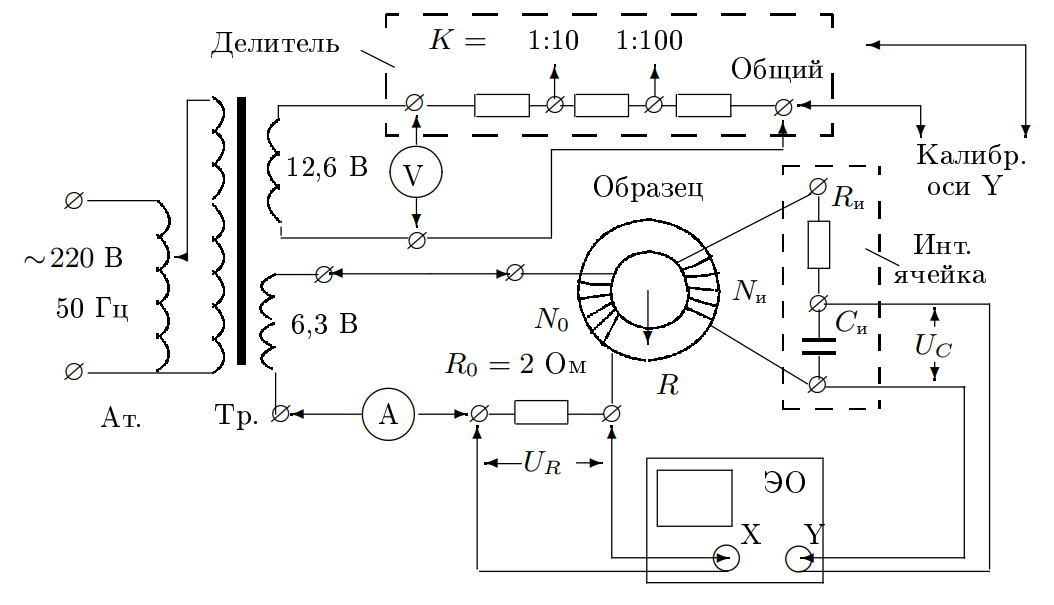
\includegraphics[width=5in]{scheme.png}
\caption{Схема экспериментальной установки.}
\label{ust}
\end{center}
\end{figure}

\medskip\hrule\medskip

\section{Экспериментальная часть}

\subsection{Измерение петли гистерезиса.}

\paragraph{} Измерим петлю гистерезиса для трёх образцов. Физические характеристики образцов:

\begin{table}[h]
\begin{center}
\begin{tabularx}{0.8\textwidth}{|l|X|X|X|}
\hline 
• & I & II & III \\ 
\hline 
Образец & Феррит 1000нн & Пермаллой (Fe-Ni НП50) & Кремнистое железо (Fe-Si) \\ 
\hline 
$N_0$, витков & 35 & 40 & 35 \\ 
\hline 
$N_U$, витков & 400 & 200 & 350 \\ 
\hline 
$S$, см$^2$ & 3.0 & 3.8 & 1.2 \\ 
\hline 
$2 \pi R$, см & 25 & 24 & 10 \\ 
\hline 
\end{tabularx} 
\caption{Физические характеристики образцов.}
\label{physchar}
\end{center}
\end{table}

\paragraph{} Пронаблюдаем петли гистерезиса для различных образцов. Наблюдения зафиксируем на рисунках (\ref{hist1}, \ref{hist2}, \ref{hist3}).

\begin{figure}
\begin{center}
\begin{minipage}[h]{7cm}
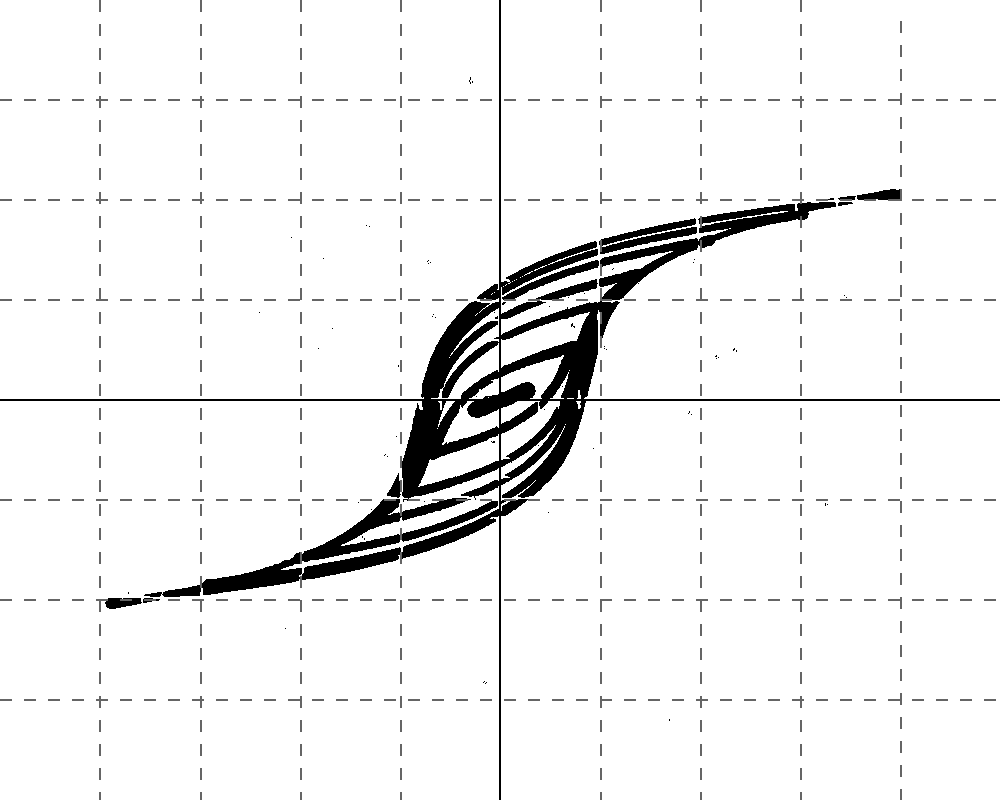
\includegraphics[width=7cm]{Hist 1.png}
\caption{Петли гистерезиса для образца I} 
\label{hist1}
\end{minipage}
\hfill
\begin{minipage}[h]{7cm}
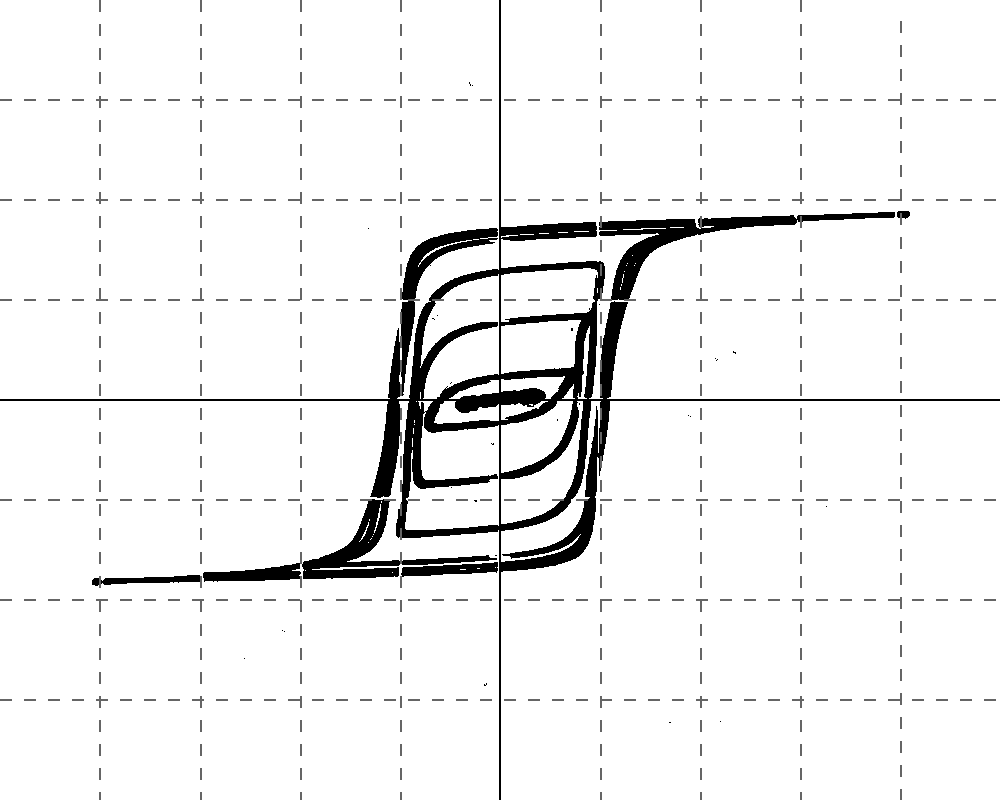
\includegraphics[width=7cm]{Hist 2.png}
\caption{Петли гистерезиса для образца II}
\label{hist2}
\end{minipage}
\end{center}
\end{figure}

\begin{figure}
\begin{center}
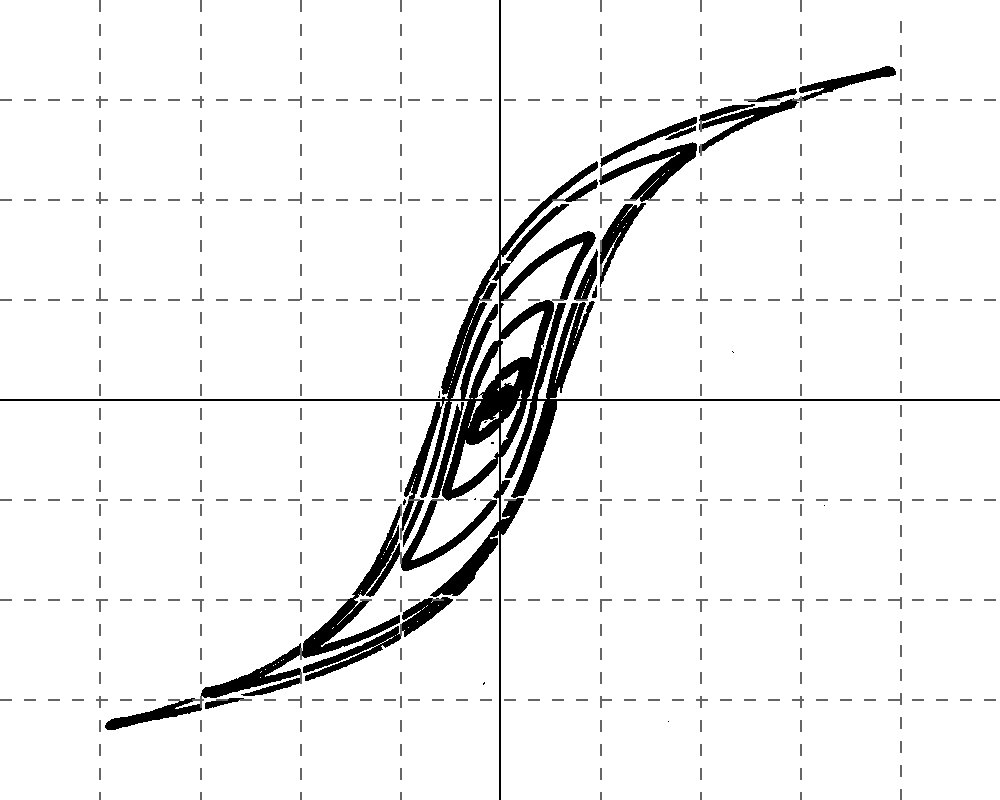
\includegraphics[width=7cm]{Hist 3.png}
\caption{Петли гистерезиса для образца III}
\label{hist3}
\end{center}
\end{figure}

\paragraph{} Для наблюдаемых петель гистерезиса запишем коэффициенты усиления $K_x$, $K_y$, силу тока в намагничивающей обмотке $I_\text{эфф}$, а также полную ширину и высоту предельной петли $2X_s, 2Y_s$, и двойные амплитуды коэрцитивного поля $2X_c$ и остаточной индукции $2Y_r$.

\begin{table}[h]
\begin{center}
\begin{tabularx}{0.8\textwidth}{|l|X|X|X|}
\hline
Образец & I & II & III \\
\hline
$K_x$, мВ/дел & 20 & 50 & 100 \\ \hline
$K_y$, мВ/дел & 20 & 100 & 50 \\ \hline
$I_{\max}$, мА & 159 & 293 & 798 \\ \hline
$2X_s$, дел & 7.93 & 8.20 & 7.79 \\ \hline
$2Y_s$, дел & 4.19 & 3.76 & 6.74 \\ \hline
$2X_c$, дел & 1.67 & 2.34 & 1.23 \\ \hline
$2Y_r$, дел & 2.38 & 3.44 & 2.83 \\ \hline
\end{tabularx}
\caption{Наблюдения петли гистерезиса.}
\label{histtable}
\end{center}
\end{table}


\subsection{Калибровка осциллографа}

\paragraph{} Чувствительность осциллографа по осям $Ox$ и $Oy$ рассчитаем по формулам:
\[ m_x = \frac{2 \sqrt{2} R_0 I_\text{эфф}}{2x}, \; m_y = \frac{2 \sqrt{2} U_\text{эфф}}{2y}.
\]
Для этого измерим $I_\text{эфф}$ и $2x$ для различных значений чувствительности оси $Ox$ и $U_\text{эфф}$ и $2y$ для различных значений чувствительности оси $Oy$. Подставим измеренные значения в формулы (чувствительность записана в круглых скобках):

\[ m_x = \frac{2 \sqrt{2} \cdot 0.3 \text{Ом} \cdot 0.89 \text{А}}{8} = 94.4 \text{мВ/дел (100 мВ)}, \]
\[ m_x = \frac{2 \sqrt{2} \cdot 0.3 \text{Ом} \cdot 0.449 \text{А}}{8} = 47.6 \text{мВ/дел (50 мВ)}, \]
\[ m_x = \frac{2 \sqrt{2} \cdot 0.3 \text{Ом} \cdot 0.181 \text{А}}{8} = 19.2 \text{мВ/дел (20 мВ)}, \]
\[ m_y = \frac{2 \sqrt{2} \cdot 0.137 \text{В}}{4} = 96.9 \text{мВ/дел (100 мВ)}, \]
\[ m_y = \frac{2 \sqrt{2} \cdot 0.105 \text{В}}{6} = 49.5 \text{мВ/дел (50 мВ)}, \]
\[ m_y = \frac{2 \sqrt{2} \cdot 0.0401 \text{В}}{8} = 18.9 \text{мВ/дел (20 мВ)}. \]

\subsection{Определение параметров RC-ячейки}

\paragraph{} Подадим на вход интегрирующей ячейки напряжение $U_\text{вх}$ и измерим напряжение на выходе $U_\text{вых}$. Рассчитаем постоянную времени по формуле:
 \[ \tau_\text{и} \approx \frac{U_\text{вх}}{\omega_0 U_\text{вых}} = \frac{6 \text{В}}{2 \pi \cdot 50 \text{Гц} \cdot 44 \text{мВ}} \approx 0.43 \text{с}. \]
Рассчитаем постоянную времени по значениям указанных на ячейке:
\[ \tau = RC = 20 \text{кОм} \cdot 20 \text{мкФ} = 0.4 \text{с}. \]
Видим, что рассчитанное значение близко к измеренному.

\subsection{Обработка результатов}

\paragraph{} Рассчитаем Коэффициенты отклонений по осям X-Y в напряжённость $H$ и индукцию  $B$ пользуясь рассчитанными в п.п. ii данными для чувствительности и формулами:

\[ H = \frac{IN_0}{2 \pi R}, \; I = \sqrt{2} I_\text{эфф}, \; |B| = \frac{\tau_\text{и}}{SN_U} U, \; U = m_y \cdot Y. \]

Пользуясь данными из таблиц (\ref{physchar}, \ref{histtable}) вычислим значения для:

\[ H_{\max} = \frac{N_0 I_{\max} \sqrt{2}}{2 \pi R}, \; B_s = \frac{\tau m_y 2Y_s}{2SN_U}, \; H_c = H_{\max} \frac{2X_s}{2X_c}, \; B_r = B_s \frac{2Y_s}{2Y_r}.
\]

\begin{table}[h]
\begin{center}
\begin{tabularx}{0.8\textwidth}{|l|X|X|X|}
\hline
Образец & I & II & III \\ \hline
$H_{\max}$, А/м & 31.5 & 69.1 & 395.0 \\ \hline
$B_s$, Тл & 0.132 & 0.959 & 1.589 \\ \hline
$H_c$, А/м & 6.63 & 19.7 & 62.4 \\ \hline
$B_r$, Тл & 0.075 & 0.811 & 0.667 \\ \hline
\end{tabularx}
\caption{Рассчитанные характеристики образцов.}
\end{center}
\end{table}


Из вычислений восстановим предельную петлю гистерезиса и начальную кривую намагничивания. Проведём касательные к восстановленной кривой намагничивания в начальной точке, и точке с максимальным наклоном. По наклону касательной оценим начальное и максимальное значение дифференциальной магнитной проницаемости.

\begin{figure}
\begin{center}
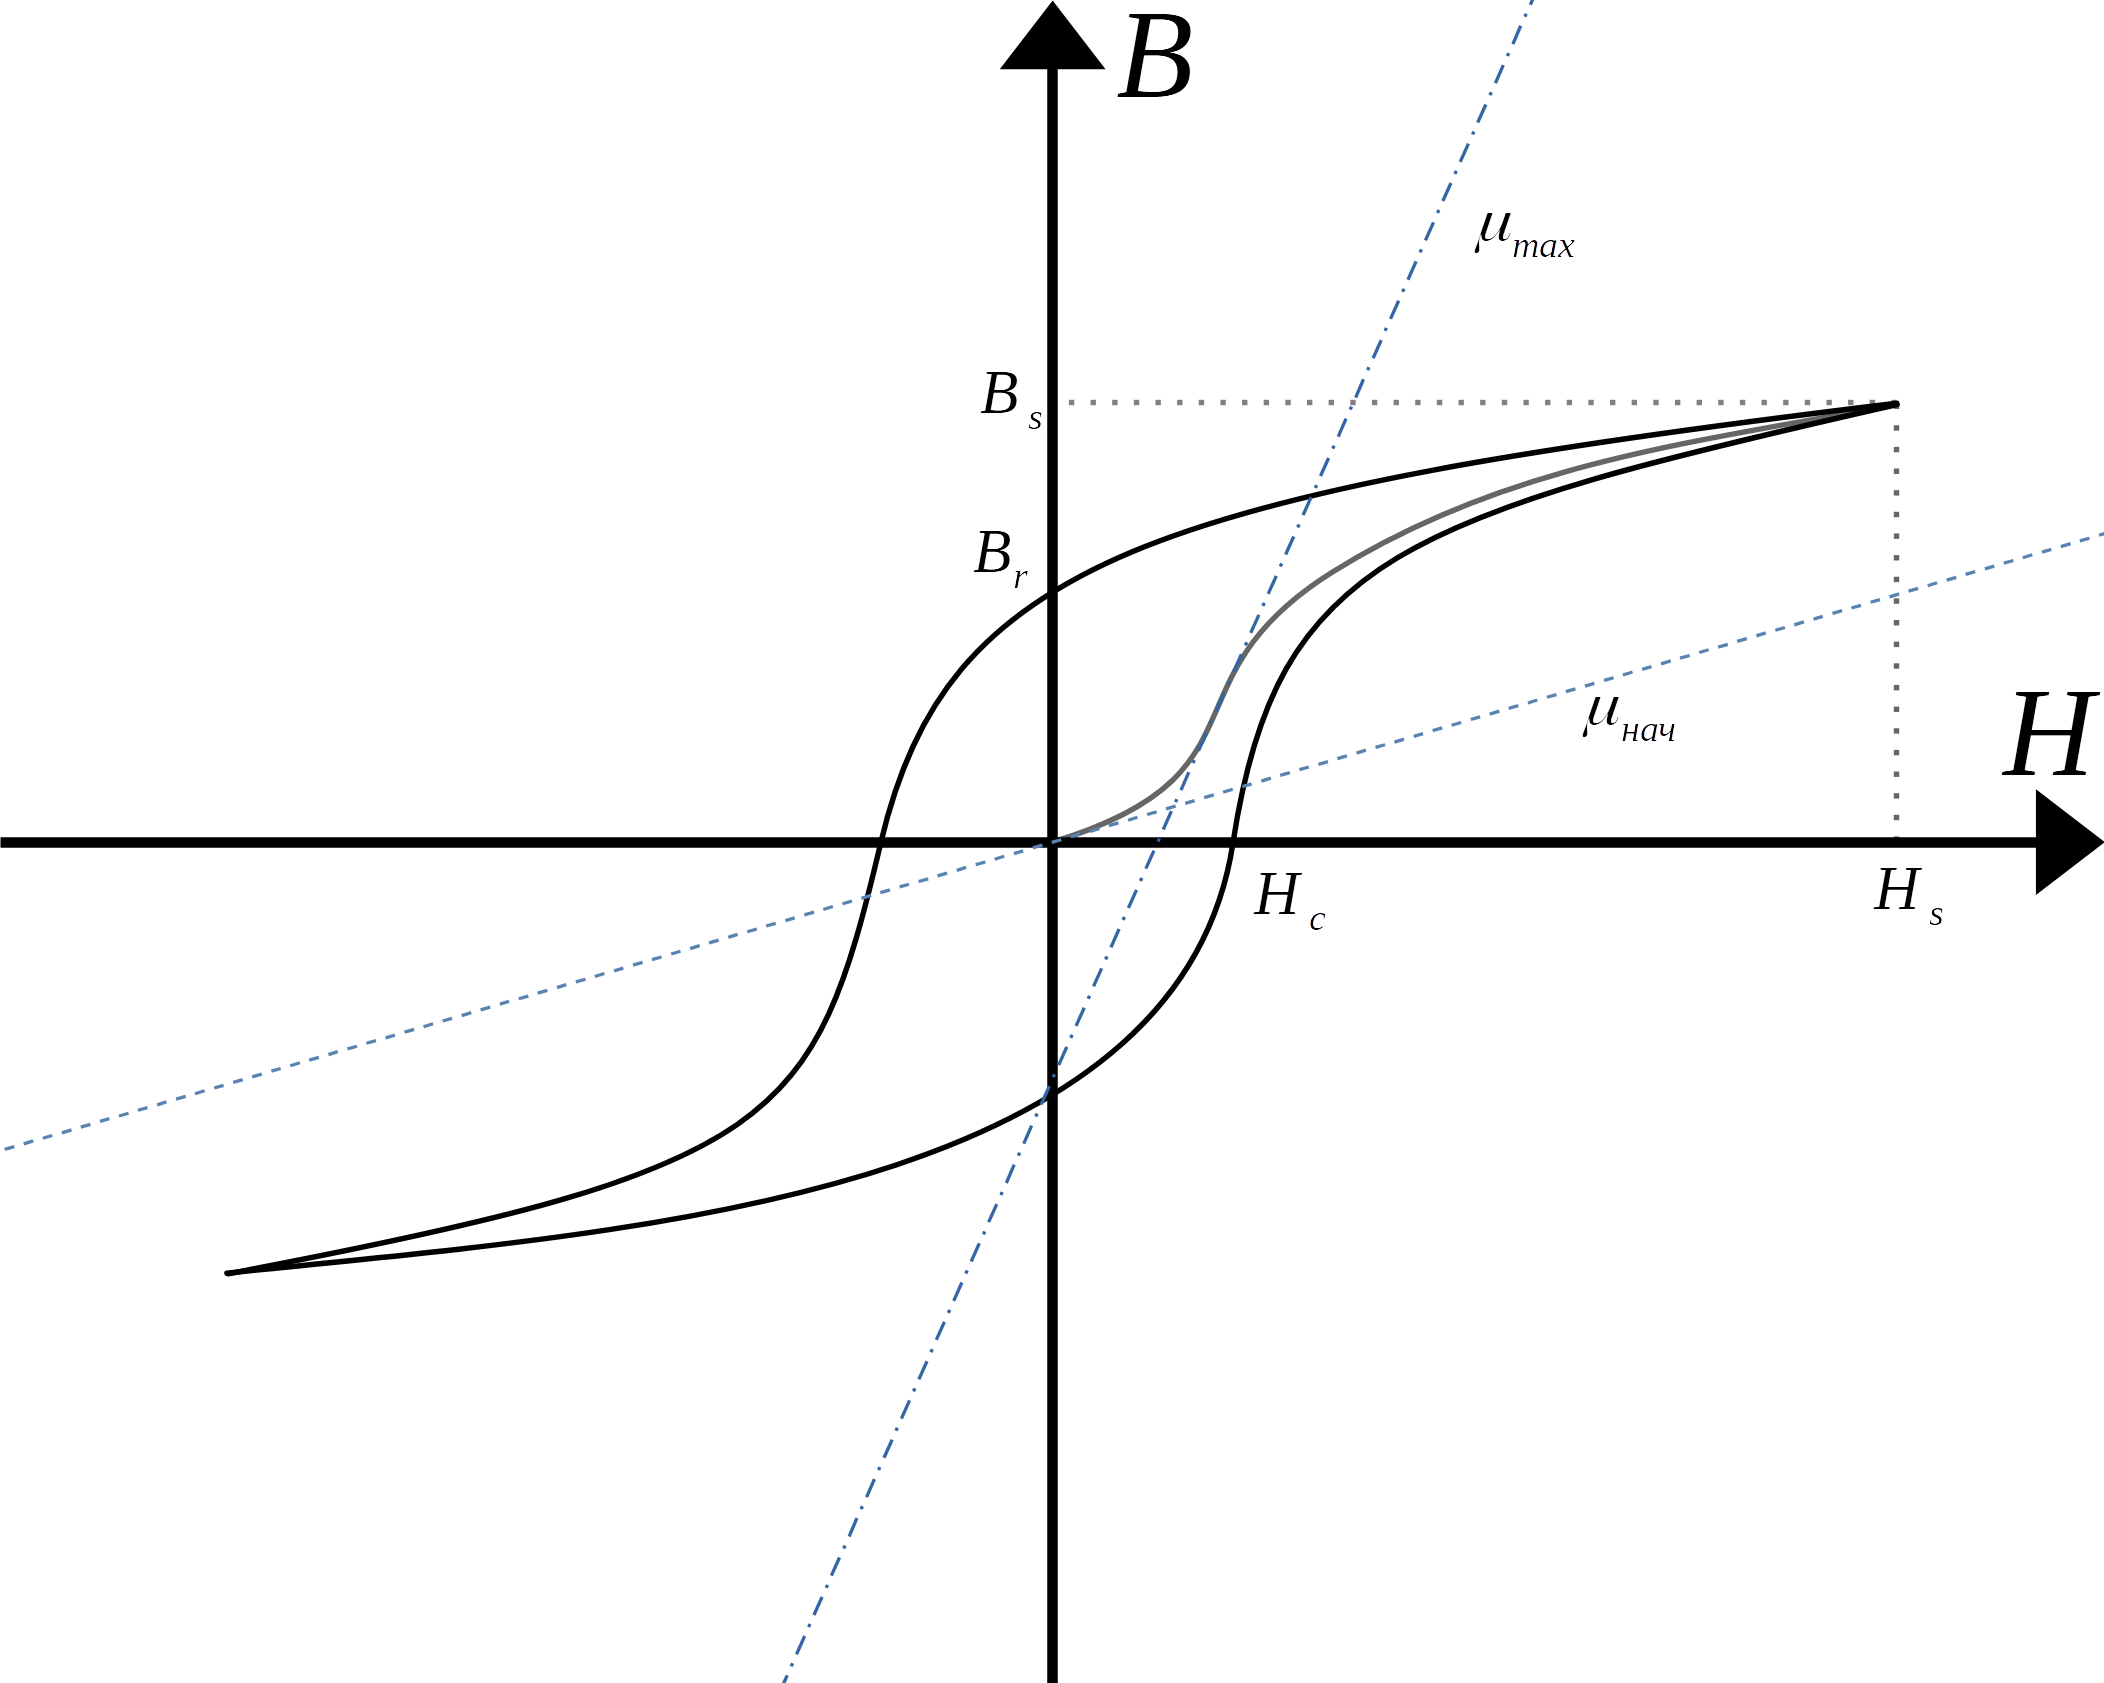
\includegraphics[width=5in]{hist graph 1.png}
\caption{Предельная петля гистерезиса и начальная кривая намагничивания для образца I} 
\label{hist1}
\end{center}
\end{figure}

\begin{figure}
\begin{center}
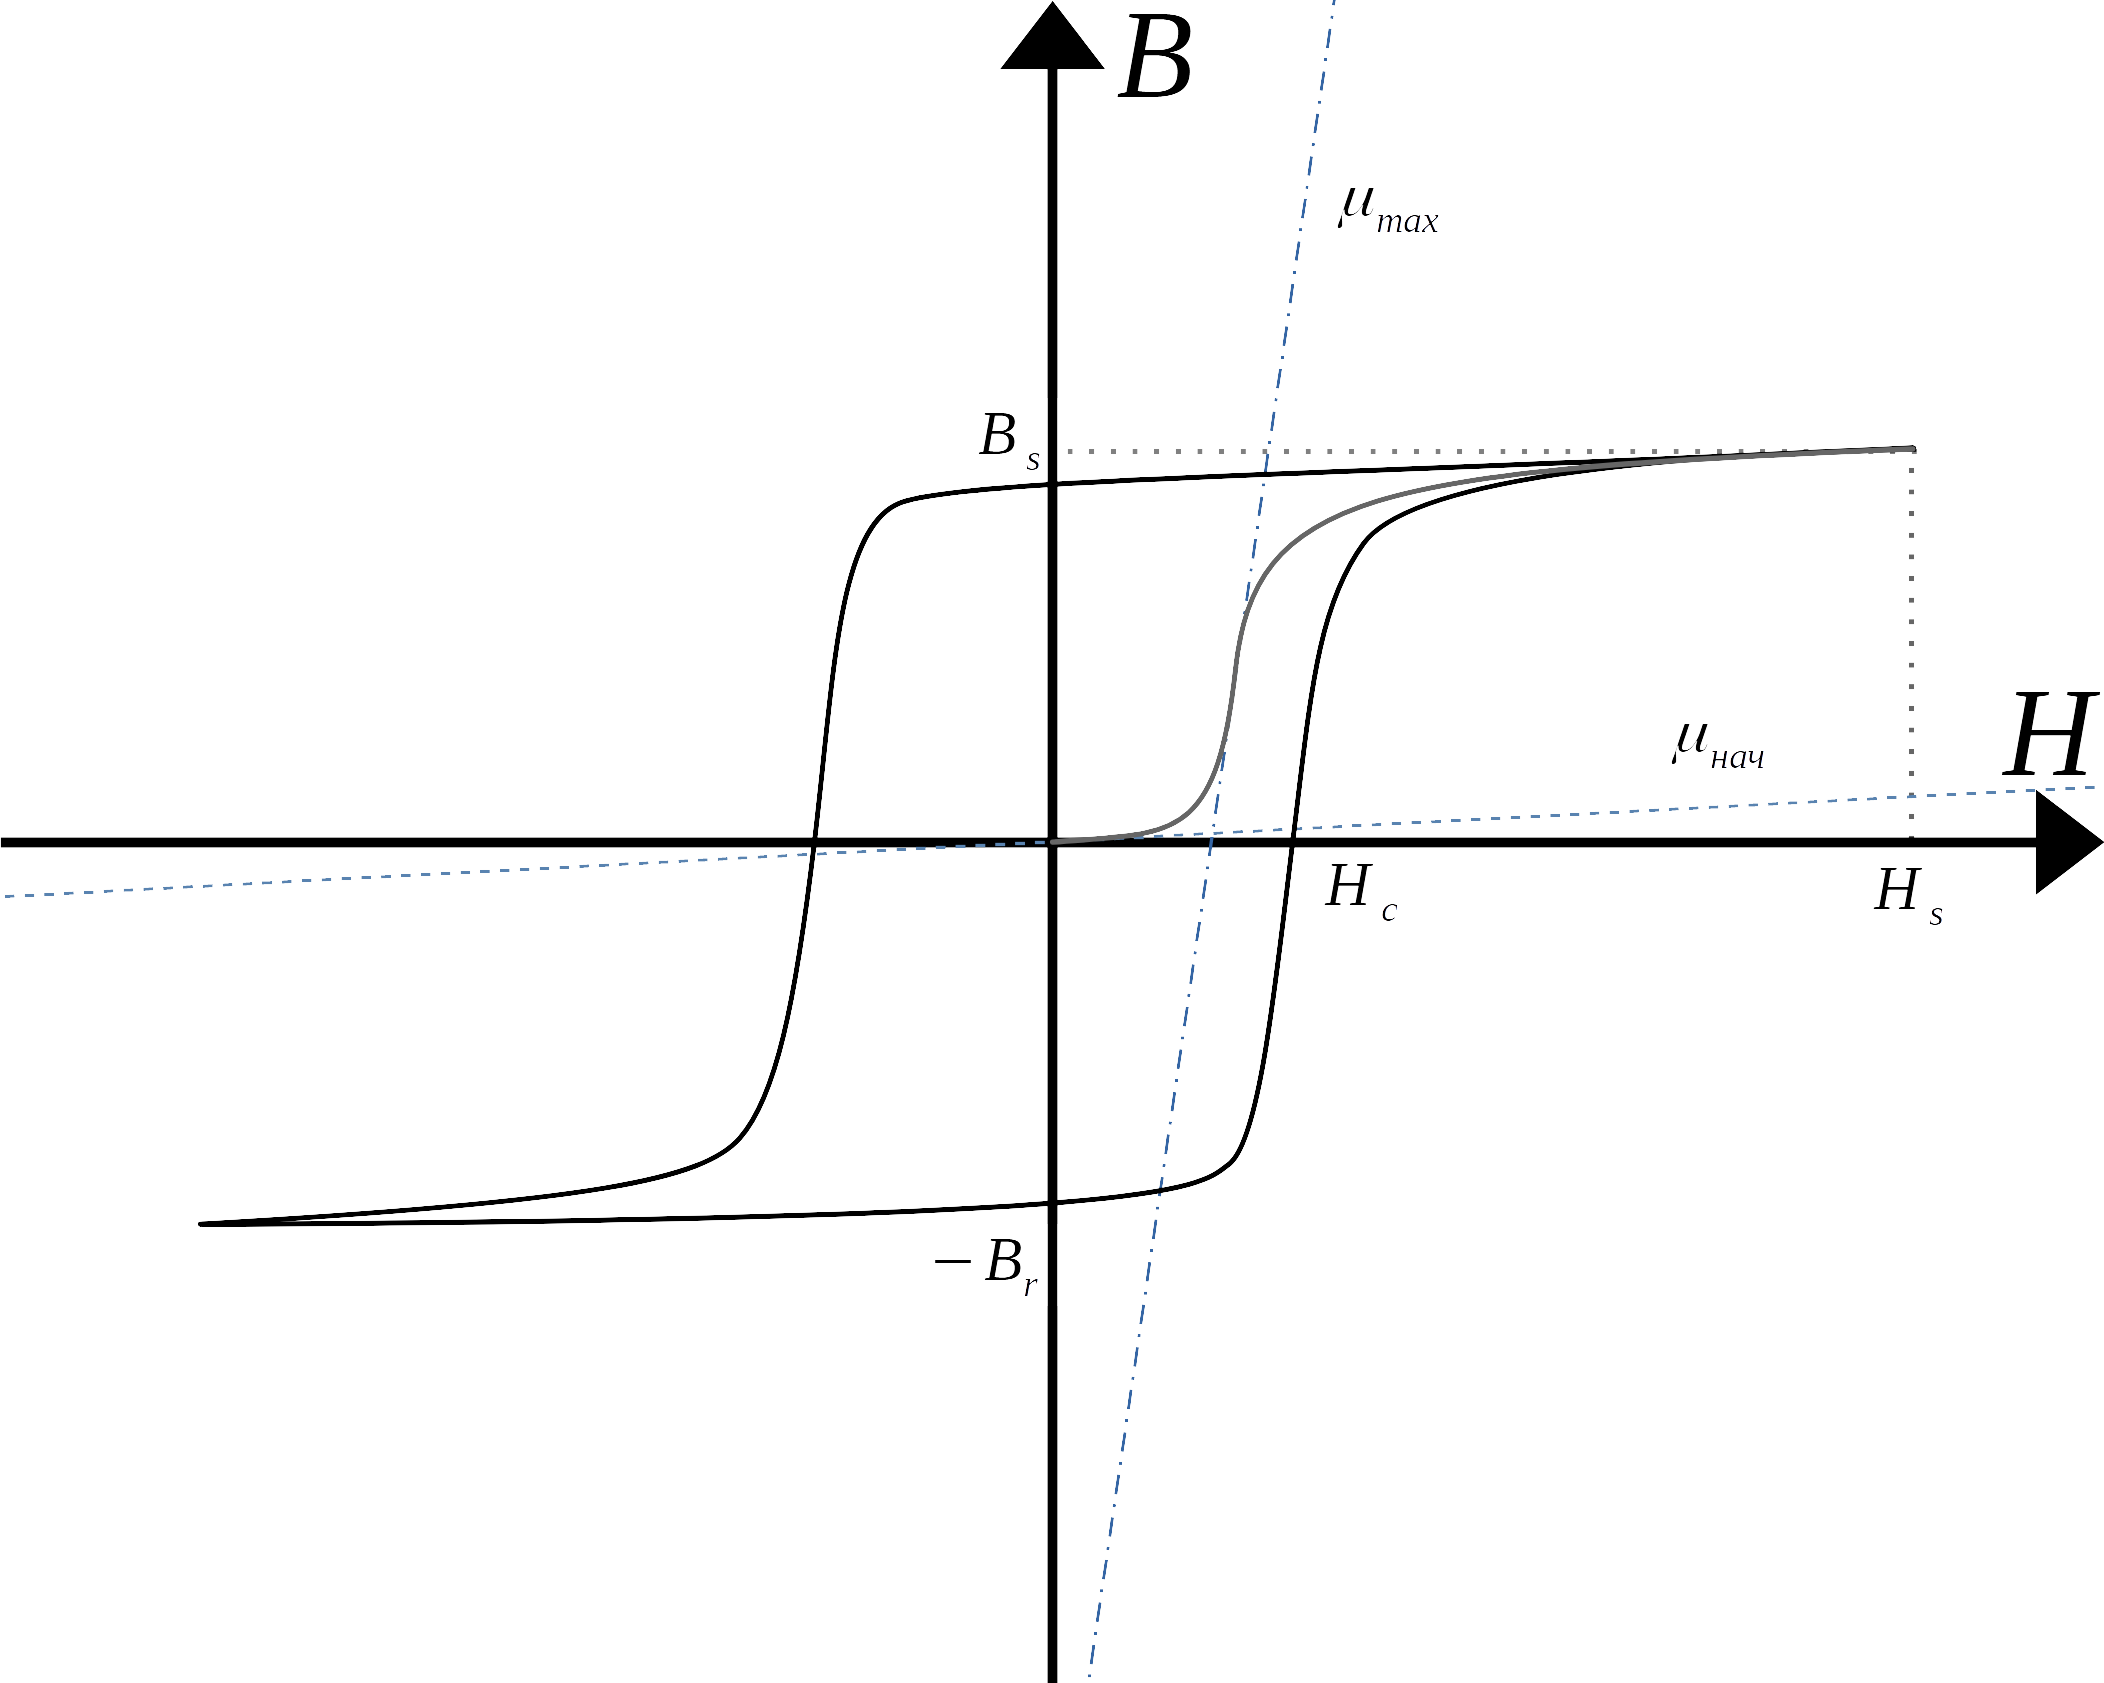
\includegraphics[width=5in]{hist graph 2.png}
\caption{Предельная петля гистерезиса и начальная кривая намагничивания для образца II} 
\label{hist2}
\end{center}
\end{figure}

\begin{figure}
\begin{center}
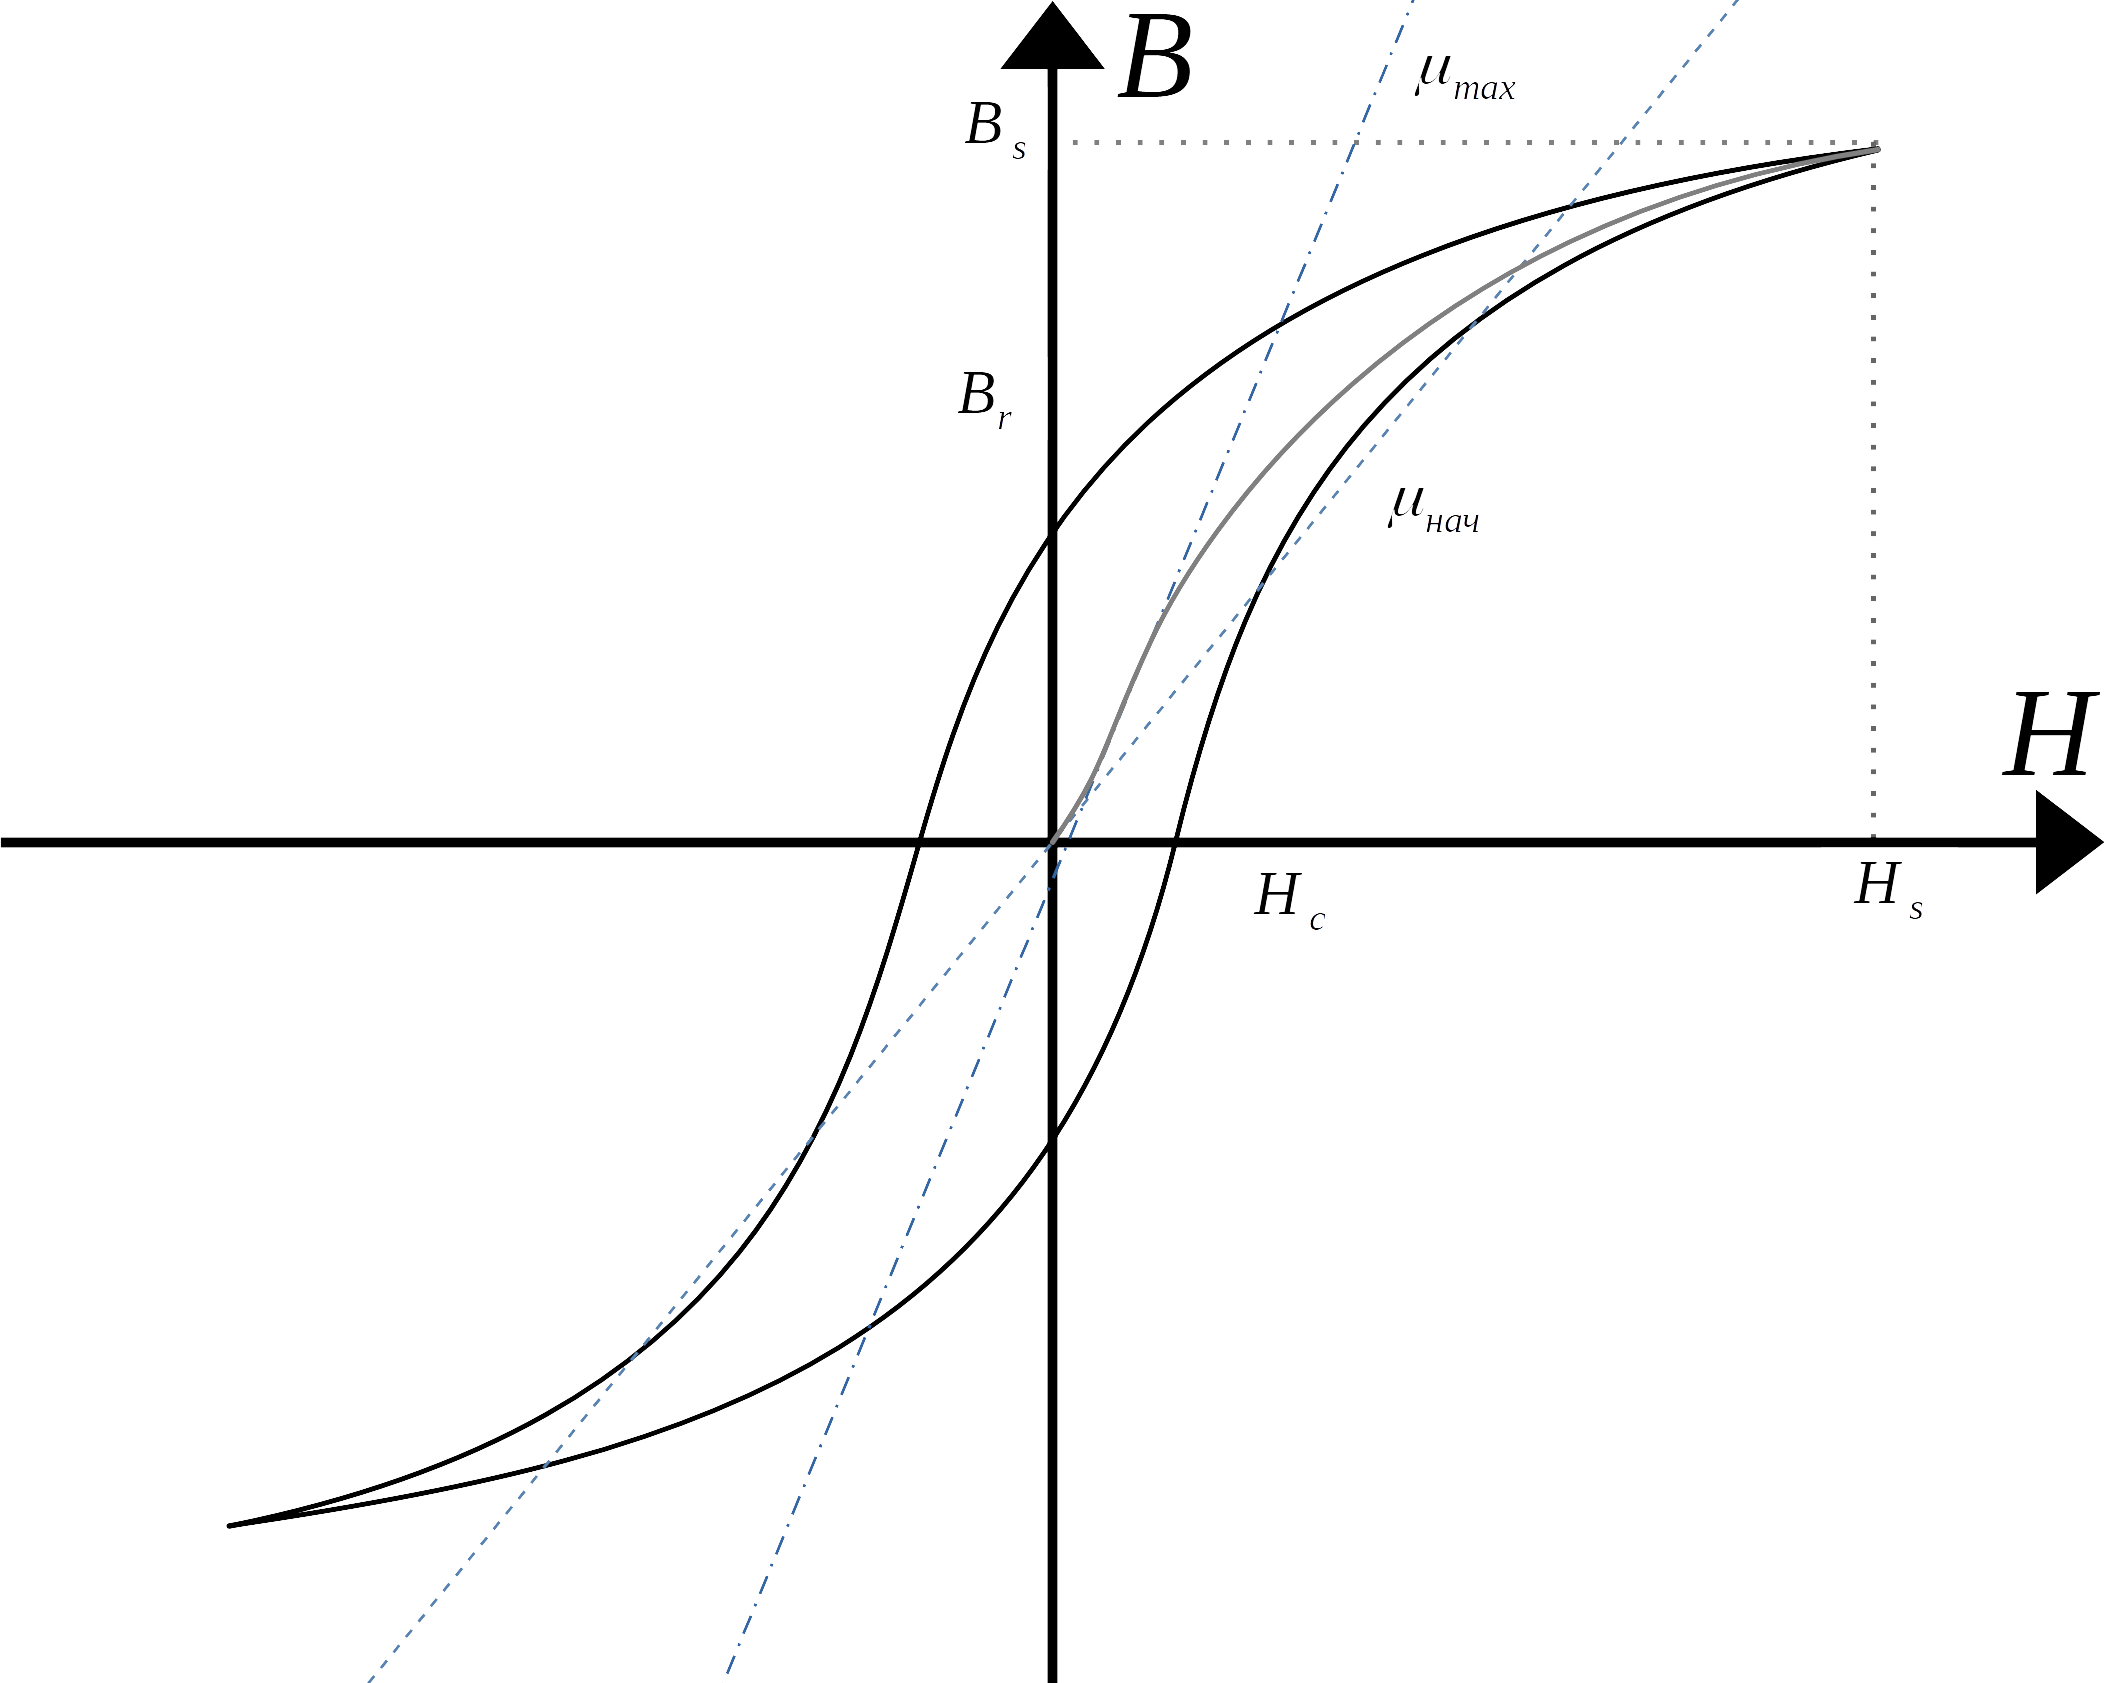
\includegraphics[width=5in]{hist graph 3.png}
\caption{Предельная петля гистерезиса и начальная кривая намагничивания для образца III} 
\label{hist3}
\end{center}
\end{figure}

\begin{table}
\begin{center}
\begin{tabularx}{0.8\textwidth}{|l|X|X|X|}
\hline
Образец & I & II & III \\ \hline
$\mu_\text{нач}$, Гн/м & $2.3 \cdot 10^{-3}$ & $1.6 \cdot 10^{-3}$ & $5.5 \cdot 10^{-3}$ \\ \hline
$\mu_\text{нач} / \mu_0$ & 1800 & 1200 & 4400 \\ \hline
$\mu_\text{max}$, Гн/м & $1.8 \cdot 10^{-2}$ & $0.19$ & $1.1 \cdot 10^{-2}$ \\ \hline
$\mu_\text{max} / \mu_0$ & $1.4 \cdot 10^{4}$ & $1.5 \cdot 10^{5}$ & $8 \cdot 10^{3}$ \\ \hline

\end{tabularx}
\caption{Значение дифференциальной магнитной проницаемости.}
\end{center}
\end{table}

\subsection{Оценка погрешностей и полученных результатов.}

\paragraph{} На точность измерений влияет несколько факторов:

\begin{itemize}
\item Счёт данных через осциллограф -- экран осциллографа не всегда способен передать точные численные данные.
\item Влияние измерительных устройств -- при высоких токах из-за переключения режима амперметра искажалась петля, видимая на экране осциллографа.
\item Работа с восстановленным графиком -- восстановленный график может отличатся от действительного.
\end{itemize} 

Всё вышеперечисленное делает данные перечислены возможным расчёт значений лишь в пределах порядка.

\medskip\hrule\medskip

\section{Выводы}

\paragraph{} Нам удалось при помощи электронного осциллографа пронаблюдать явление гистерезиса, и качественно показать различия между свойствами ферромагнетиков, а именно изменение формы кривой гистерезиса.

\paragraph{} При помощи наблюдаемых кривых мы смогли оценить величины коэрцитивного поля $H_c$, индукции насыщения $B_S$, магнитной проницаемости $\mu_\text{нач}$ и $\mu_\text{max}$ с точностью до порядка, чем показали, что данный метод можно применять с некоторой эффективностью.


\medskip\hrule\medskip

\end{document}
